\subsection{Problem 1}
\subsubsection{Decomposition rate model}

By consulting relevant data and analyzing, it can be found that the main factors affecting the decomposition rate include temperature, humidity, overlap degree between communities, oxygen concentration, illumination intensity, time, woody plant species, site, years decayed, mesh, sampling side, extension rate, etc. Therefore, we can take the above influencing factors as independent variables, and choose the decomposition rate as the dependent variable to describe the breakdown of ground litter and woody fibers, and start to establish the decomposition rate model.

It is assumed that there are $k$ independent variables. Firstly, each independent variable is quantified, normalized and dimensionless, and the category variable needs dummy element processing. Then, in the case of known data of $N$ groups of $k$ independent variables, the decomposition rate's approximate equation of each independent variable is selected as follows:
\begin{equation}\label{1.1}
    y^{*}=a_{0}+a_{1}x_{1}+\dots+a_{k}x_{k}
\end{equation}
Where,

$y^{*}$ is the approximate value of $y$;

$x_{i}$ is the value of the i-th influencing factor, namely the i-th independent variable;

$a_{i}$ is the assumed coefficient, $i=0, 1, \dots, k$.

In the case of known data of $N$ groups of $k$ independent variables, the minimum sum of squares of the deviation between the measured value and the calculated value is taken as the "optimization criterion". Let:
\begin{equation}\label{1.2}
    \varphi(a_{0},a_{1},\dots\,a_{k})=\sum_{n = 1}^{N}(y_{n}-y_{n}^{*})^{2}=\sum_{n = 1}^{N} (y_{n}-a_{0}-a_{1}x_{1n}-\dots-a_{k}x_{kn})^{2}
\end{equation}

Where,

$y_{n}$ is the decomposition rate under the data of the nth group;

$y_{n}^*$ is the approximate value of the decomposition rate under data of the nth group;

$x_{in}$ is the ith independent variable under the data of the nth group.

The least square method is used to determine all the coefficients in Equation (\ref{1.1}):

Through the method of finding the extreme value of the multivariate function, take the partial derivative in Equation (\ref{1.2}) and make it equal to zero, so as to reach the minimum value. For $k+1$ partial derivatives are as follows:
\begin{equation}\label{}
\left\{
\begin{array}{l}
    \frac{\partial \varphi}{\partial a_{0}} = -2\sum_{n = 1}^{N} (y_{n}-a_{0}-a_{1}x_{1n}-\dots-a_{k}x_{kn})=0 \\
    \frac{\partial \varphi}{\partial a_{1}} = -2\sum_{n = 1}^{N} (y_{n}-a_{0}-a_{1}x_{1n}-\dots-a_{k}x_{kn})x_{1n}=0 \\
    \dots \\
    \frac{\partial \varphi}{\partial a_{k}} = -2\sum_{n = 1}^{N} (y_{n}-a_{0}-a_{1}x_{1n}-\dots-a_{k}x_{kn})x_{kn}=0 \\
\end{array}
\right.
\end{equation}

By transforming the above equation, we get:
\begin{equation}\label{}
\left\{
\begin{array}{l}
    Na_{0}+\sum_{n = 1}^{N}a_{1}x_{1n}+\dots+\sum_{n = 1}^{N}a_{k}x_{kn}=\sum_{n = 1}^{N}y_{n} \\

    \sum_{n = 1}^{N}a_{0}x_{1n}+\sum_{n = 1}^{N}a_{1}x_{1n}x_{1n}+\dots+\sum_{n = 1}^{N}a_{k}x_{kn}x_{1n}=\sum_{n = 1}^{N}y_{n}x_{1n} \\

    \dots \\

    \sum_{n = 1}^{N}a_{0}x_{kn}+\sum_{n = 1}^{N}a_{1}x_{1n}x_{kn}+\dots+\sum_{n = 1}^{N}a_{k}x_{kn}x_{kn}=\sum_{n = 1}^{N}y_{n}x_{kn} \\
\end{array}
\right.
\end{equation}

After further simplification, we can get:
\begin{equation}\label{1.4}
\left\{
\begin{array}{l}
    a_{1}l_{11}+a_{2}l_{12}+\dots+a_{k}l_{1k}=l_{1y} \\
    a_{1}l_{21}+a_{2}l_{22}+\dots+a_{k}l_{2k}=l_{2y} \\
    \dots \\
    a_{1}l_{k1}+a_{2}l_{k2}+\dots+a_{k}l_{kk}=l_{ky} \\
\end{array}
\right.
\end{equation}

\begin{equation}\label{1.5}
    a_{0}=\bar{y}-a_{1}\bar{x_{1}}-\dots-a_{k}\bar{x_{k}}
\end{equation}

Where,
\begin{equation}\label{}
\left\{
\begin{array}{l}
    l_{ij}=l_{ji}=\sum_{n = 1}^{N}x_{in}x_{jn}-\frac{1}{N}(\sum_{n = 1}^{N}x_{in})(\sum_{n = 1}^{N}x_{jn})  \\
    l_{iy}=\sum_{n = i}^{N}y_{n}x_{in}-\frac{1}{N}(\sum_{n = 1}^{N}x_{in})(\sum_{n = 1}^{N}x_{jn})  \\
    i=1,2,\dots,k; j=1,2,\dots,k; \\
\end{array}
\right.
\end{equation}

According to the above transformation, as long as the relevant variables satisfy the Equation (\ref{1.4}) and Equation (\ref{1.5}), the minimum value of $\varphi (a_{0},a_{1},\dots,a_{k})$ can be obtained. So we can determine all the coefficients by solving Equation (\ref{1.4}) and Equation (\ref{1.5}). Then, the decomposition rate can be obtained as follows:

\begin{equation}\label{}
    y=f(x_{1},x_{2},\dots,x_{k})=a_{0}+a_{1}x_{1}+\dots+a_{k}x_{k}
\end{equation}

\subsubsection{Solution of Problem 1}

By analyzing the data provided by Nicky Lustenhouwer\upcite{Lustenhouwer11551}, we draw four violin maps to analyze the relationship between the Mass loss and Site, Years decayed, Mesh and Sampling side.
\begin{figure}[H]
    \centering
    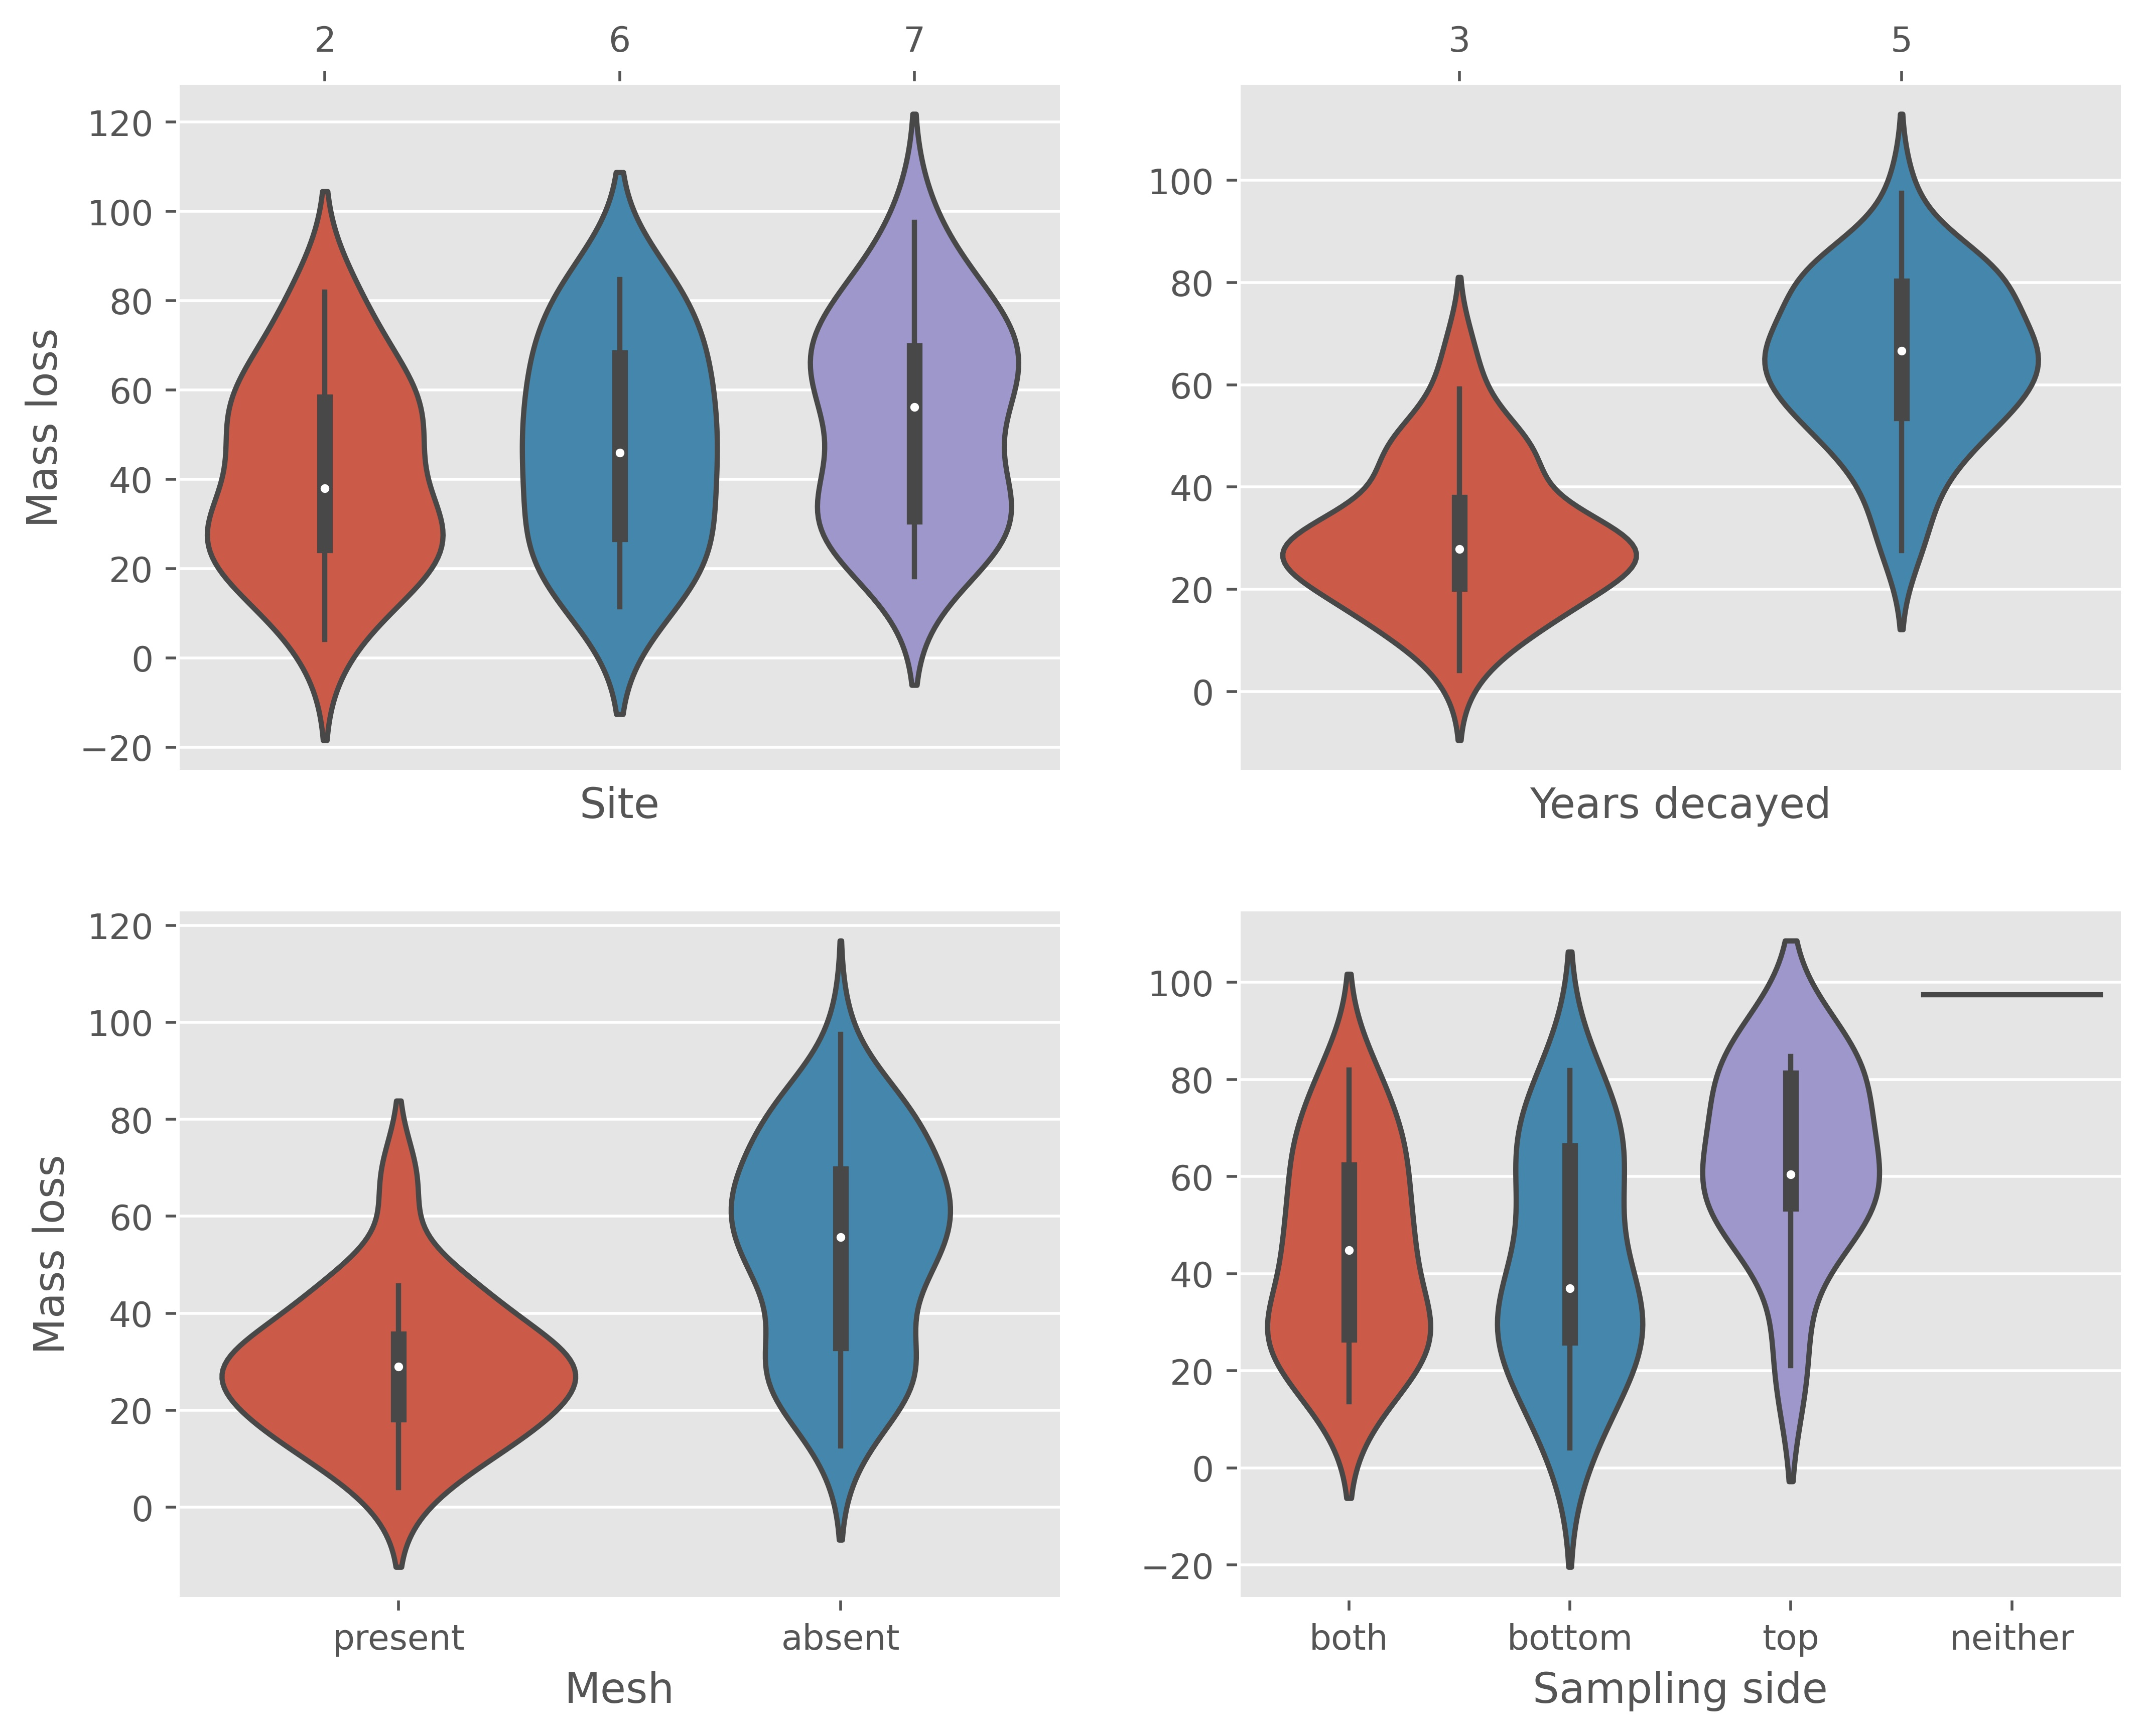
\includegraphics[width=0.6\textwidth]{./code/fig1.jpg}
    \caption{Violin maps between Mass loss and other variables}\label{fig1}
\end{figure}

Among the four maps showed in Figure (\ref{fig1}), we can find clearly the close connection between Mass loss and Years decayed. So we explore the linear relationship between Mass loss and Extension rate grouped by Years decayed as follows:
\begin{figure}[H]
    \centering
    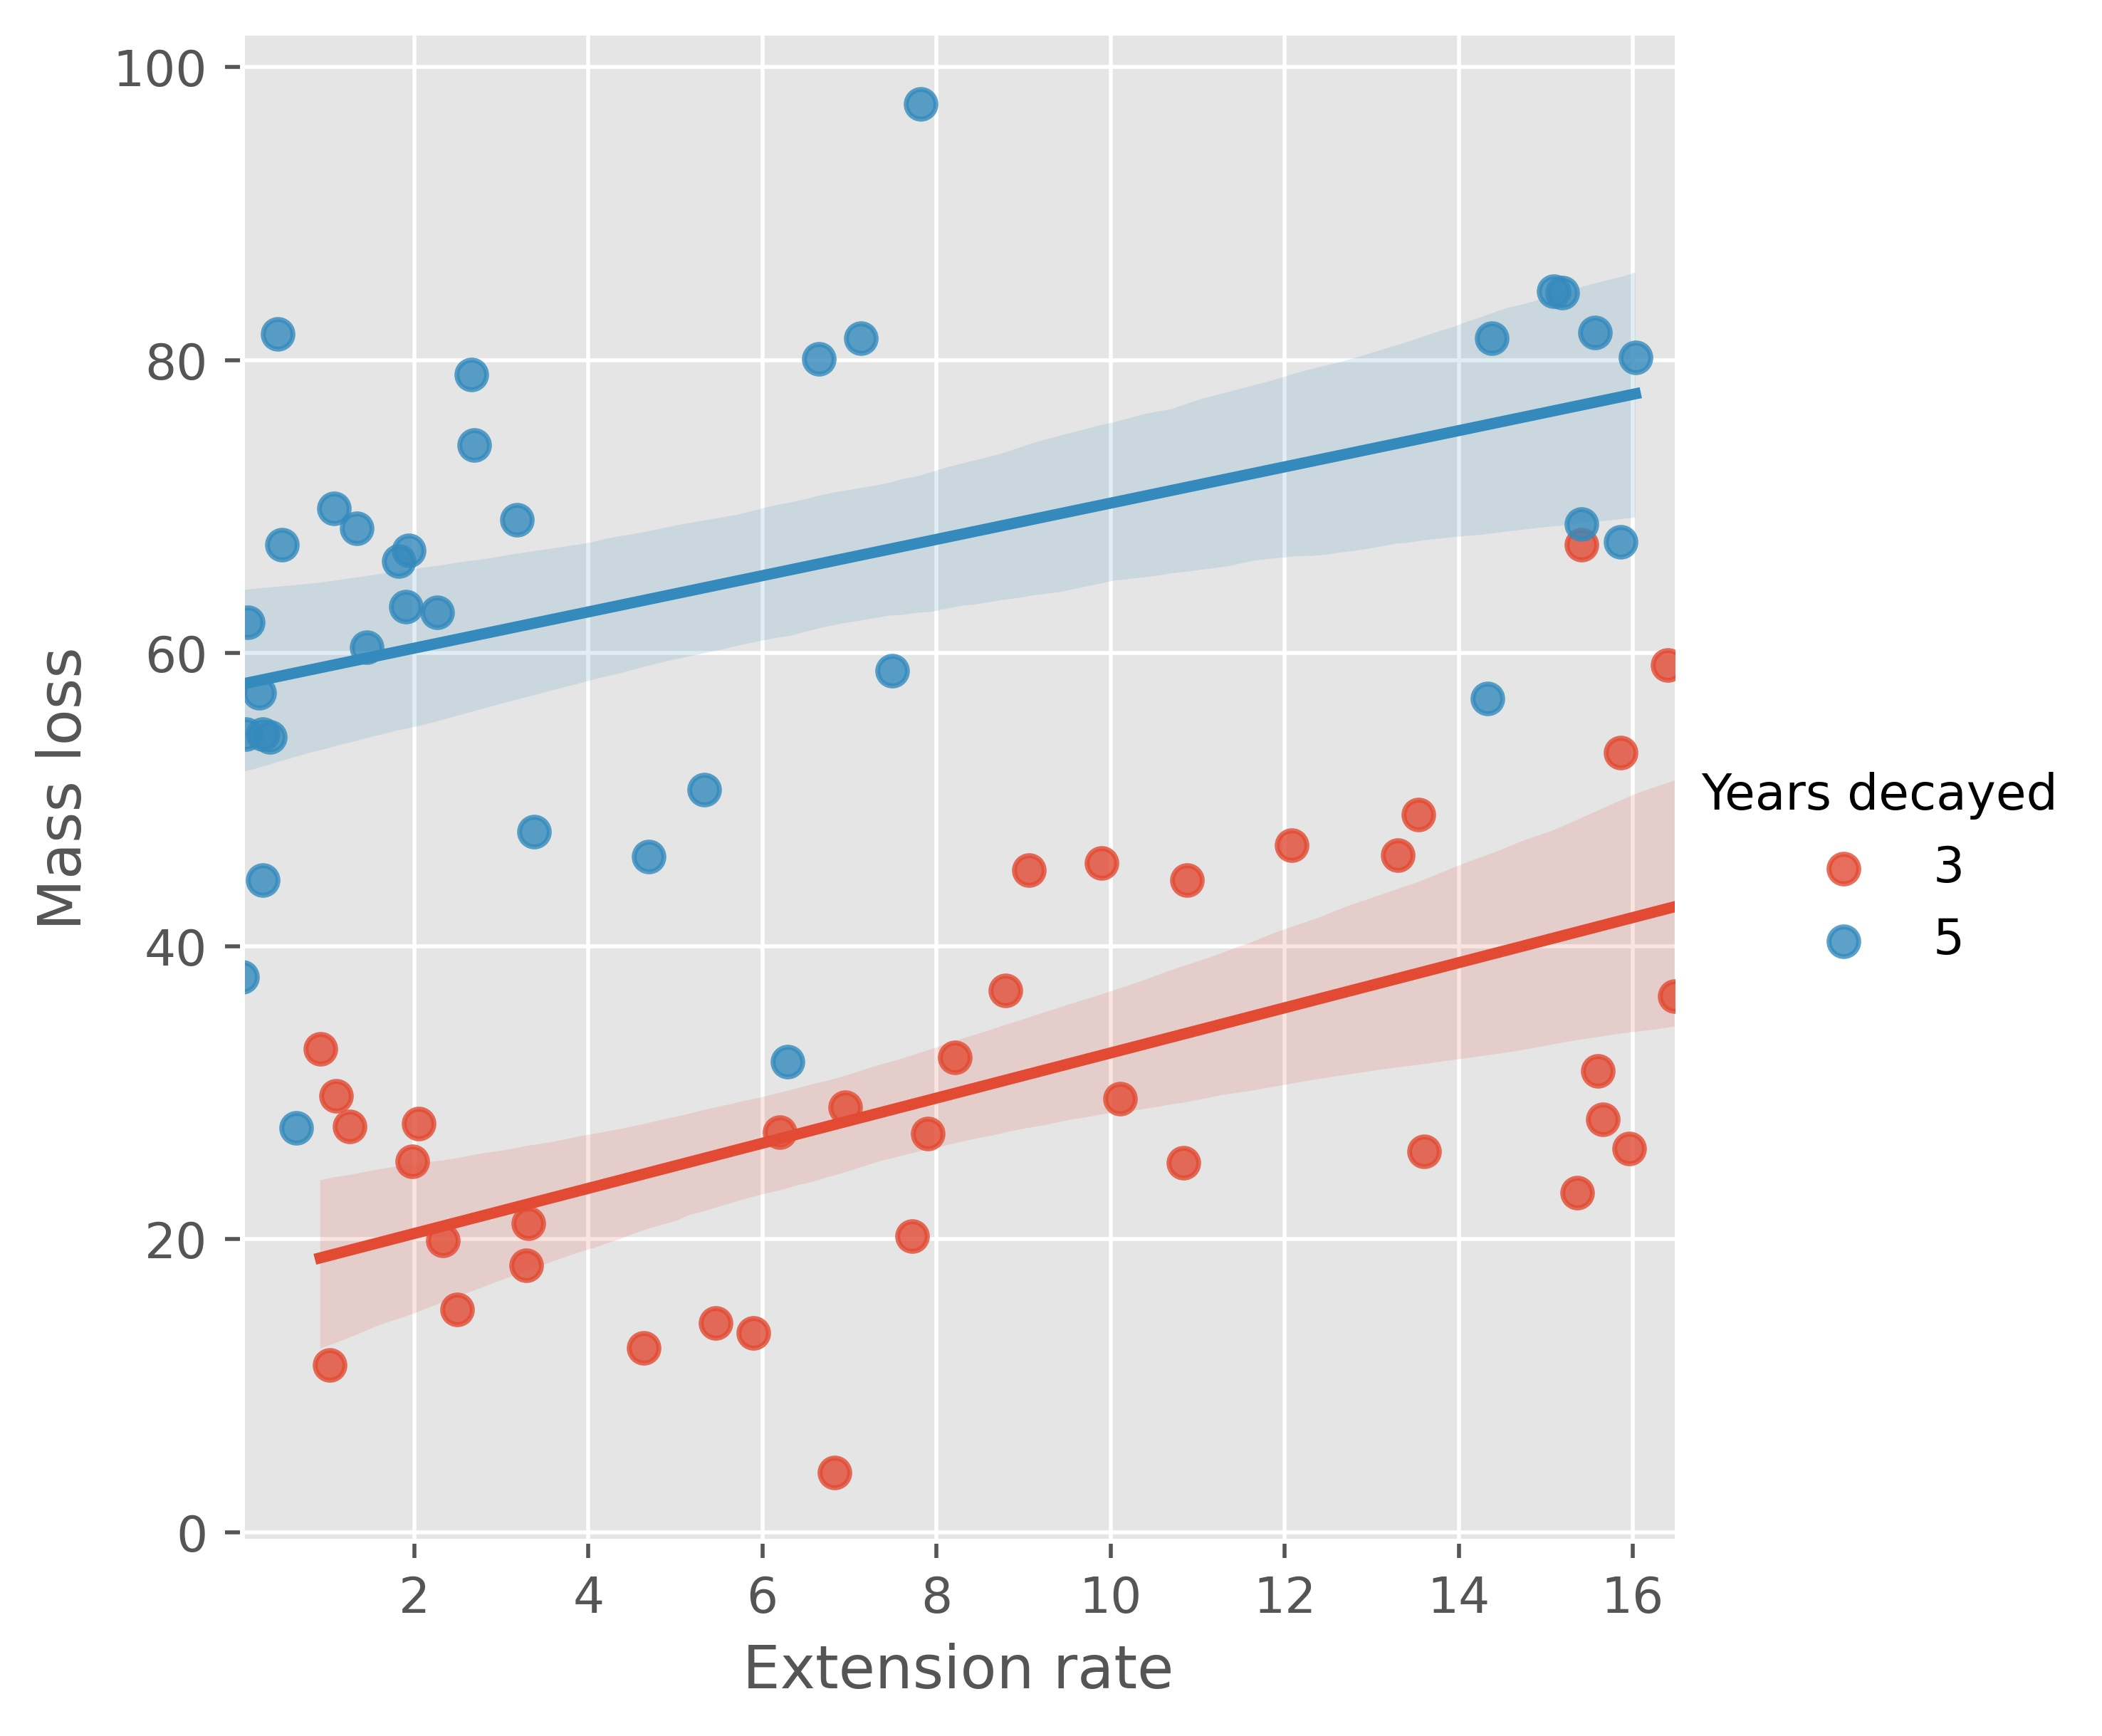
\includegraphics[width=0.65\textwidth]{./code/fig2.jpg}
    \caption{Linear relationship between Mass loss and Extension rate}\label{fig2}
\end{figure}

Using the least square method, we can get the function expression of Mass loss regarding Extension rate under different Years decayed conditions as follows:

\begin{equation}\label{}
\left\{
\begin{array}{l}
    y=1.54x+17.31, when\ c = 3; (R^2=0.34)\\
    y=1.237x+57.87, when\ c = 5; (R^2=0.20) \\
\end{array}
\right.
\end{equation}

Where,

$y$ is Mass loss;

$x$ is Extension rate;

$c$ is Years decayed.

$R^2$ is the coefficient of determination.